% !TEX encoding = UTF-8
% !TEX TS-program = pdflatex
% !TEX root = ../tesi.tex

%**************************************************************
\chapter{Processo di sviluppo}
\label{cap:processi-metodologie}
%**************************************************************

Durante lo sviluppo di un progetto \textit{software} è importante aderire ad un modello di \glossaryItem{ciclo di vita}. La durata del ciclo di vita di un \textit{software} inizia dalla sua concezione, ossia il momento in cui nasce il bisogno, passa poi per lo sviluppo e l'utilizzo, prolungato nel tempo e in cui è soggetto a manutenzione, per poi terminare con il ritiro del prodotto. L'avanzamento tra questi stati avviene tramite l'esecuzione di attività definite nel modello di ciclo di vita adottato. I progetti in cui non viene adottato un modello di ciclo di vita sono detti \glossaryItem{code-n-fix} e l'insieme delle attività è priva di organizzazione e rende il progetto caotico e poco gestibile. Aderire ad un modello di ciclo di vita è quindi essenziale ma determina vincoli sulla pianificazione e sulla gestione di progetto, per cui è importante che la scelta del modello da adottare avvenga prima della pianificazione del progetto. In un modello di ciclo di vita le attività sono coese e raggruppate in processi e gli ingressi e le uscite di ciascuna attività sono identificati, al fine di permettere un ordinamento temporale tra esse.

%**************************************************************
\section{Modello incrementale}

Durante il corso di Ingegneria del \textit{Software} sono stati studiati vari modelli di ciclo di vita. In particolare, viste le modalità di interazione e le richieste del \textit{tutor} aziendale, per il progetto di \textit{stage} poteva essere adottato un modello incrementale o una metodologia \glossaryItem{Agile}. Non avendo l'azienda imposto un processo di sviluppo, lo stagista ha optato per il modello incrementale in quanto già utilizzato durante il progetto di Ingegneria del \textit{Software}. Tale modello segue un approccio adattativo dove la realtà è considerata imprevedibile e per questo risulta utile nel caso in cui i requisiti possano cambiare in corso d'opera. Il modello presenta una fase iniziale di analisi e progettazione dove il problema viene compreso nel suo contorno fondamentale individuando i requisiti macroscopici e l'architettura del prodotto. Tale fase non viene ripetuta e risulta essenziale per la pianificazione dei cicli di incremento in cui si decide il numero di incrementi necessari a soddisfare i requisiti e si associano i requisiti ai vari incrementi pianificati. In seguito alla pianificazione è possibile transitare nella fase di realizzazione che comprende attività di progettazione in dettaglio e codifica. Tale fase è incrementale e al termine di ogni incremento si verifica che tutti i requisiti associati ad esso siano stati soddisfatti. Se la verifica va a buon fine è possibile integrare l'incremento con quanto già stato prodotto nelle fasi precedenti, costruendo in questa maniera una nuova \glossaryItem{baseline} di prodotto. Viene presentata di seguito una figura illustrativa del modello incrementale.

\begin{figure}[!h] 
    \centering 
    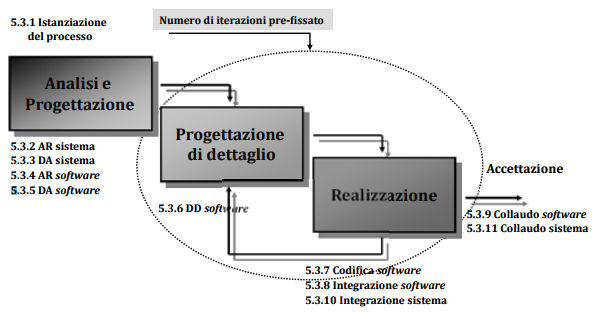
\includegraphics[width=\columnwidth]{sviluppo/ModelloIncrementale} 
    \caption{Modello di ciclo di vita incrementale}
\end{figure}

Tra i principali vantaggi di tale modello vi sono:
\begin{itemize}
	\item ogni incremento di funzionalità permette un avvicinamento alle attese e una riduzione del rischio di fallimento;
	\item le funzionalità più importanti sono le prime a raggiungere la stabilità poiché essendo inserite nei primi incrementi attraversano più cicli di verifica;
	\item il fenomeno del \glossaryItem{big-bang integration} viene evitato producendo valore ad ogni incremento;
	\item il numero di incrementi è fissato in fase di pianificazione.
\end{itemize}

Nello specifico, nella pianificazione del progetto sono stati fissati i seguenti incrementi, tutti corrispondenti ad importanti \glossaryItem{milestone} di progetto:
\begin{enumerate}
	\item realizzazione del servizio \textit{web};
	\item realizzazione della logica applicativa;
	\item realizzazione delle interfacce grafiche;
	\item stesura della documentazione annessa al progetto.
\end{enumerate}

Durante il periodo di \textit{stage} veniva pianificata una riunione con il \textit{tutor} aziendale al raggiungimento di ogni \textit{milestone}, al fine verificare che quanto prodotto nella corrispondente \textit{baseline} fosse inerente alle attese.